\documentclass{article}
\usepackage[utf8]{inputenc}
\usepackage[english]{babel}
\usepackage{fancyhdr}
\usepackage[parfill]{parskip}
\usepackage[square, numbers]{natbib}
\usepackage{appendix}
\usepackage{graphicx}
\usepackage{float}
\usepackage{amsmath}
\usepackage{amsfonts}
\usepackage{amssymb}
\usepackage{appendix}
\usepackage{listings}

\bibliographystyle{abbrvnat}
\lstset{language=Python, basicstyle=\scriptsize}

\pagestyle{fancy}
\lhead{01OVFOV}
\chead{s279331@studenti.polito.it}
\rhead{Svante Sörberg}

\title{Bioinformatics Project \#10}
\author{Svante Sörberg (s279331)}
\date{July 2020}

\begin{document}
    \thispagestyle{empty}
    \maketitle
    \begin{abstract}
        \noindent Elastic Weight Consolidation (EWC) is a technique to avoid 
        catastrophic forgetting when learning multiple tasks with a 
        neural network. In this project, EWC has been implemented on 
        a Convolutional Neural Network (CNN). The performance was studied on 
        multiple tasks in the form of permutations of the MNIST dataset. 
        The results suggest that EWC is an effective way of overcoming 
        the problem of catastrophic forgetting for a limited amount of tasks.
    \end{abstract}
    
    \clearpage
    \section*{Introduction}
        Neural networks are traditionally not well suited to multi-task 
        learning, despite being modelled after the human brain. The key
        challenge is making the neural network sensitive to the requirements
        of the new task, while not losing the ability to perform some previously
        learnt task. The problem of forgetting how to perform a previous task is 
        known as \textit{catastrophic forgetting}.

        In this project, the method of \textit{Elastic Weight Consolidation} 
        (EWC) proposed in \cite{kirkpatrick2017overcoming} is studied. 
        
        \subsection*{Background}
        The principle behind EWC is to apply a kind of regularization to the 
        weights. The most common regularization technieques penalize all 
        weights equally, usually based on how much they differ from a set value,
        typically 0 or some previously trained value for each particular weight. 
        EWC, on the other hand, penalizes weight values based on two things
        
        \begin{enumerate}
            \item The difference between value of the weight being evaluated 
        and the optimal value for that weight in previous tasks
            \item The \textit{importance} of that weight for previous tasks
        \end{enumerate}

        The idea is that weights that are important to a previously learned task
        should not be allowed to change very much. Weights that are 
        inconsequential for previous tasks may change a lot to accommodate the 
        learning of any new task. 

        \begin{figure}[H]
            \centering
            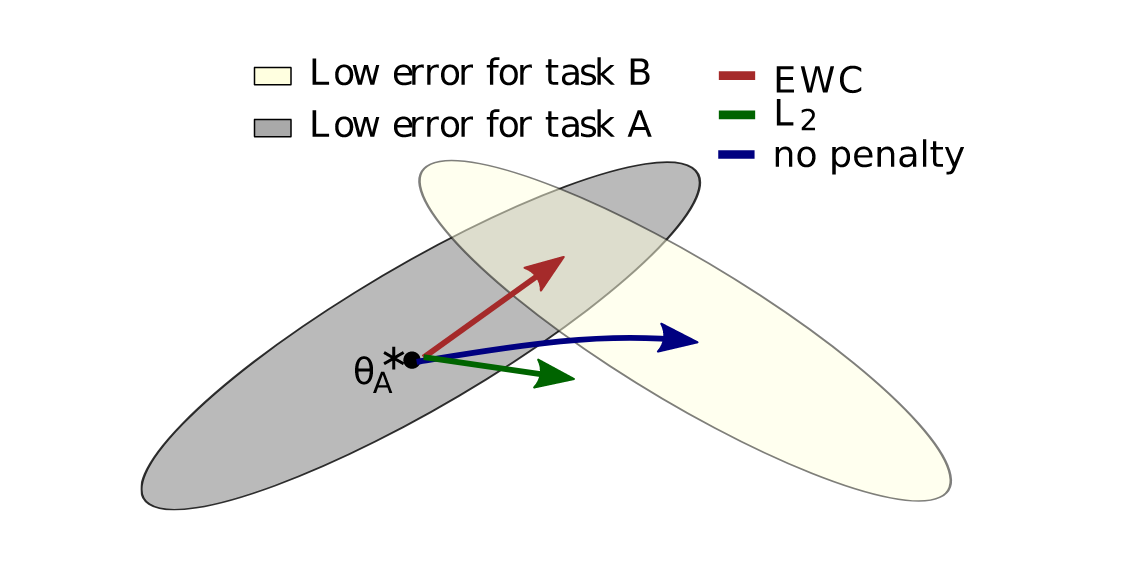
\includegraphics[width=0.6\textwidth]{figures/ewc_illustration.png}
            \caption{\textit{An illustration of EWC compared to L2-regularization and 
            no regularization. L2-regularization converges on a solution 
            in parameter space that is inbetween the optimum for the respective
            tasks. Without regularization, the weights simply change from 
            a good solution for task A, to a good solution for task B -- 
            completely forgetting task A in the process. With EWC, the parameters
            change in a direction that improves the network's ability to solve 
            task B, but maintaining them in a region where task A can still be 
            solved well. The figure is sourced from \cite{kirkpatrick2017overcoming}}}
        \end{figure}
        
        
        The ''importance'' is given by the diagonal 
        of the \textit{Fisher Information Matrix} (FIM). Without getting into 
        details, the diagonal elements of the FIM for a task K, $F_{K,i}$ can be
        approximated (in what is known as an Empirical Fisher Matrix) by 

        \begin{equation*}
            F_{A,i} = \left(\frac{\partial l(\boldsymbol{\theta})}{\partial \theta_i}\right)^2\quad
            \text{where $\theta_i$ is the i:th weight and $l(\boldsymbol{\theta})$ is the loss function}
        \end{equation*}
        
        Clearly, if $\theta_i$ is important for task A, the gradient of the loss
        (for task A) will be large (positive or negative) when taken w.r.t. 
        $\theta_i$. The full regularization term can be written as 

        \begin{equation*}
            \frac{\lambda}{2}\sum_{K}{
                \sum_{i}{F_{K,i}(\theta_i - \theta_{K,i})^2}\quad
                \text{where $\theta_{K,i}$ is the learned $\theta_i$ for task K} 
            }
        \end{equation*}

        Note that how much emphasis is put on remembering old tasks compared to 
        performing well on new ones can be controlled by the parameter $\lambda$.
        
        \subsection*{Implementation}
        The implementation more or less boils down to implementing the described 
        regularization function. At the end of the training process for each task K, the Fisher diagonal 
        $F_K$ as well as the final value for the trained parameters must be computed
        and saved, as they are needed when training subsequent tasks. 
        
        \subsection*{Experiments}
        For testing EWC, the MNIST dataset was used. To generate 
        multiple datasets of comparable difficulty, the dataset was 
        pixel-permuted, i.e. all pixels of the image shuffled without concern
        for spacial locality: 

        \begin{figure}[H]
            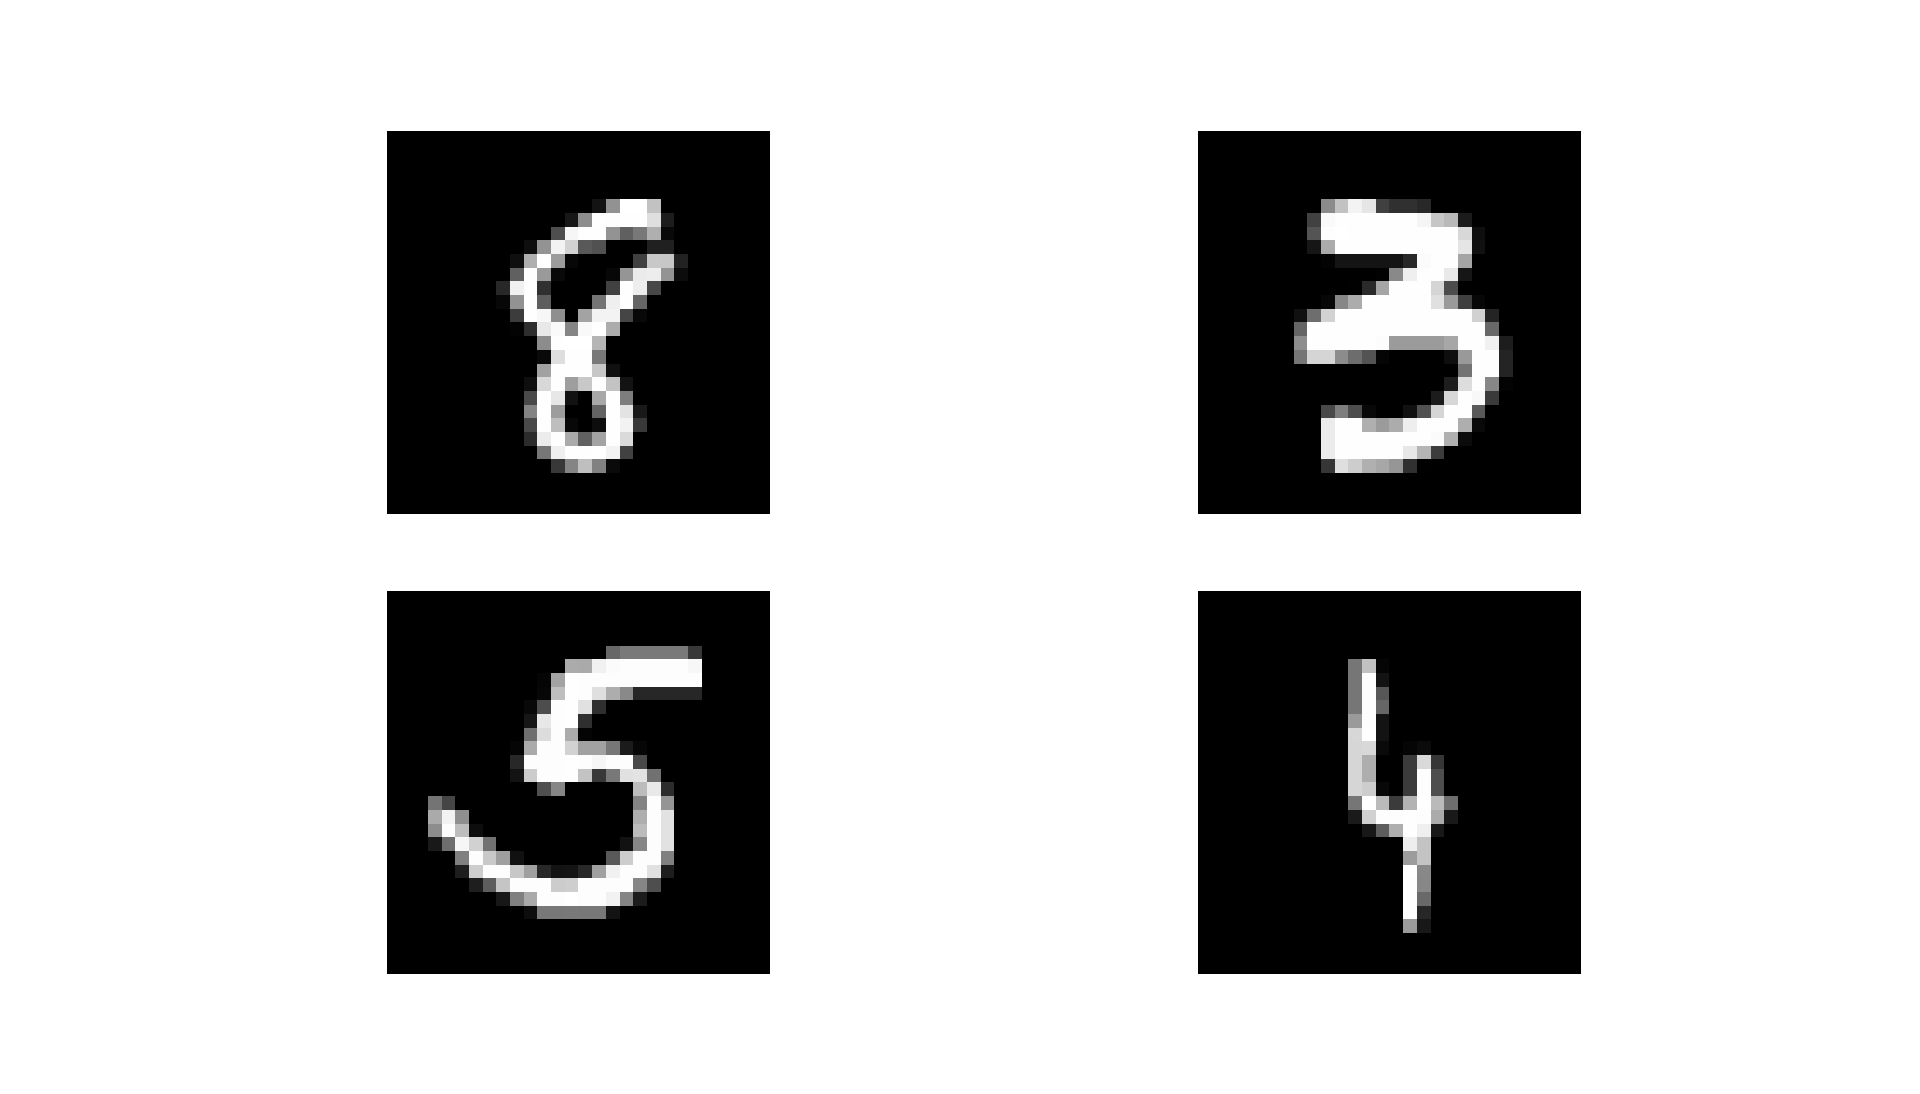
\includegraphics[width=0.49\textwidth]{figures/regular_mnist.png}
            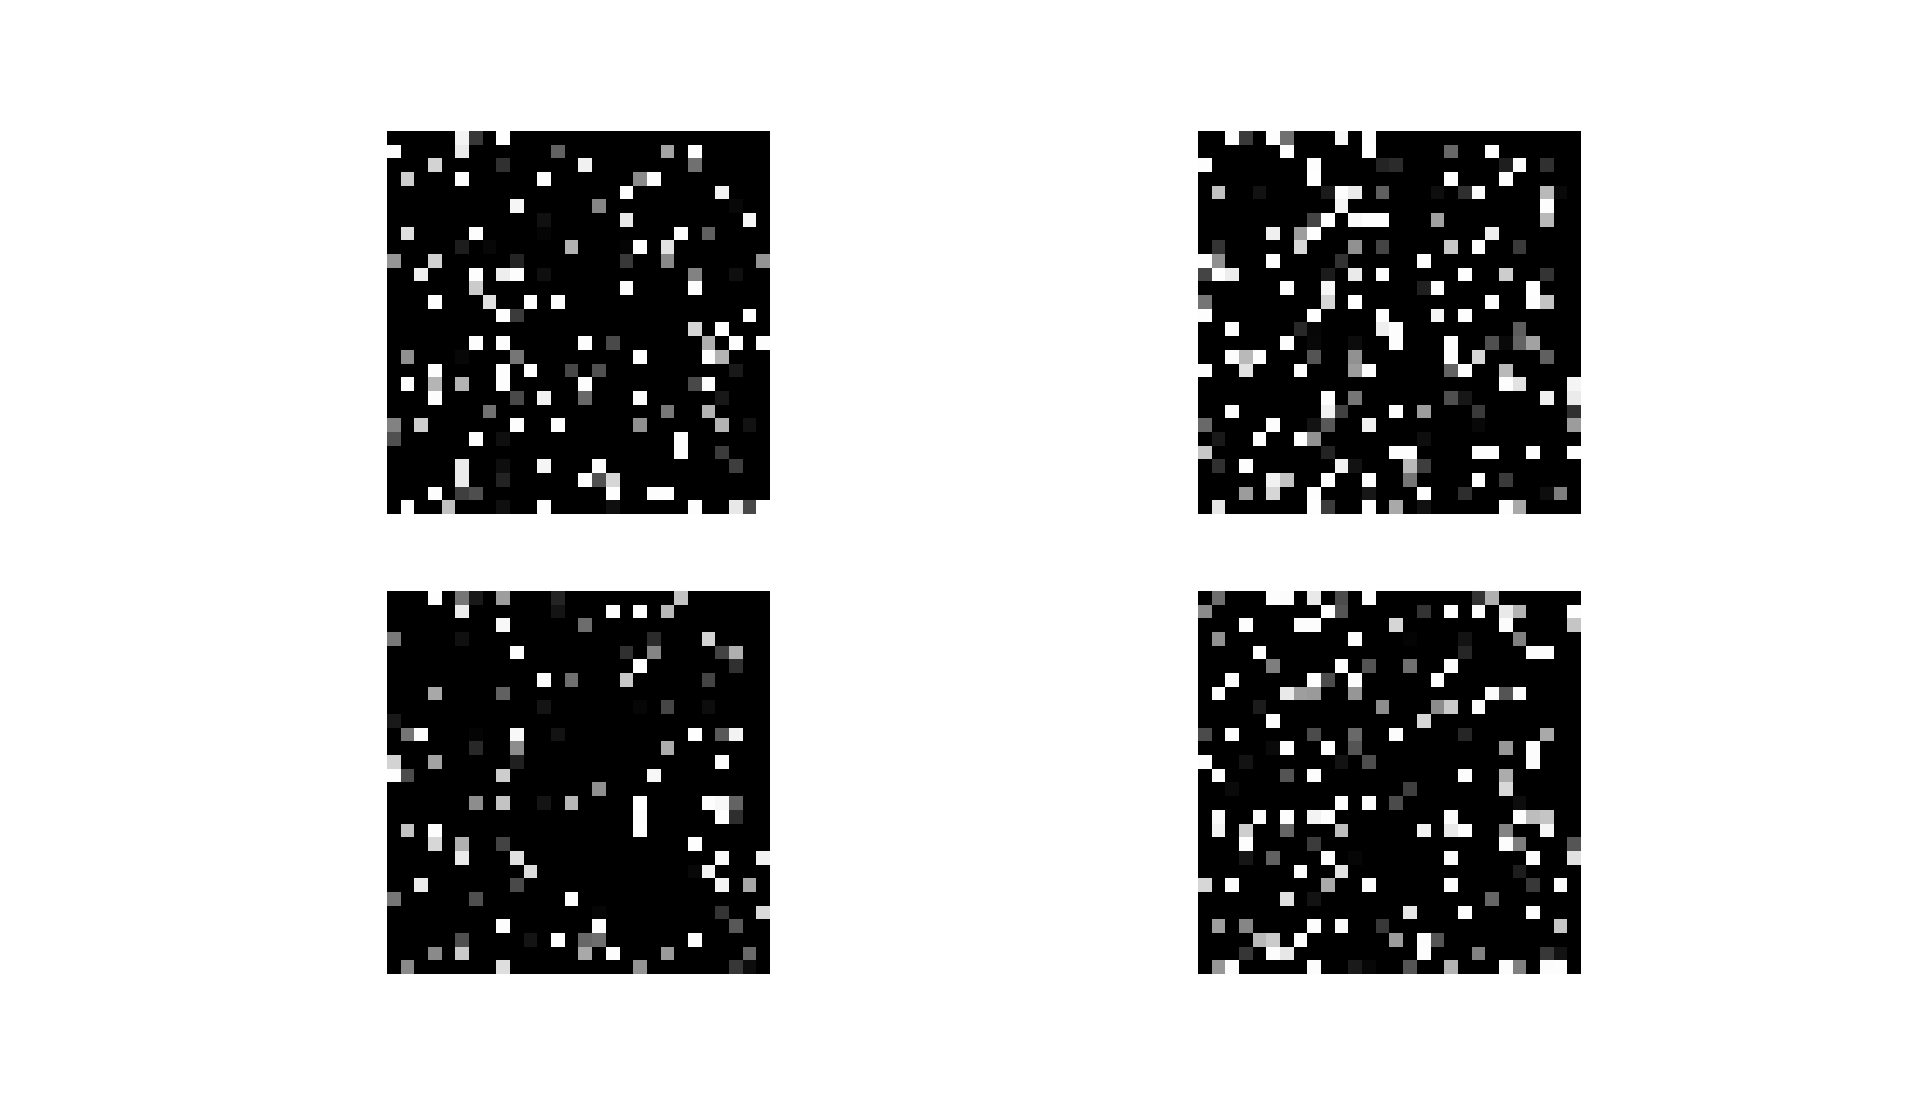
\includegraphics[width=0.49\textwidth]{figures/permuted_mnist.png}
            \caption{\textit{To the left, random images from the MNIST dataset. 
            To the right, random images from a pixel-permuted MNIST dataset.}}
        \end{figure}

        A CNN was trained, first on the regular 
        MNIST dataset, and subsequently on four permuted datasets in order for a 
        total of five different tasks. For details on the network architecture 
        and how it was trained, see appendix \ref{appendix:architecture}.
        Accuracy was recorded after each training epoch on the test set of 
        the task that was currently being trained, as well as any task that 
        the network had already been trained on.
        
        To demonstrate the problem of catastrophic forgetting, the first 
        experiment trained a network on the regular MNIST dataset. The same 
        network (without resetting weights) was then trained on all the 
        permuted MNIST datasets in sequence. There was no penalty at all for 
        diverging from the parameters learned for previous tasks. 
        For the second experiment, an EWC penalty was applied for
        all previously learned tasks. In other words, each previously learned 
        task was "kept in memory". For the third experiment, an EWC penalty was
        only applied for the previously learned task (only the previous task was 
        kept in memory).

    \section*{Results}
        \subsection*{Incremental training without penalty}
            \begin{figure}[H]
                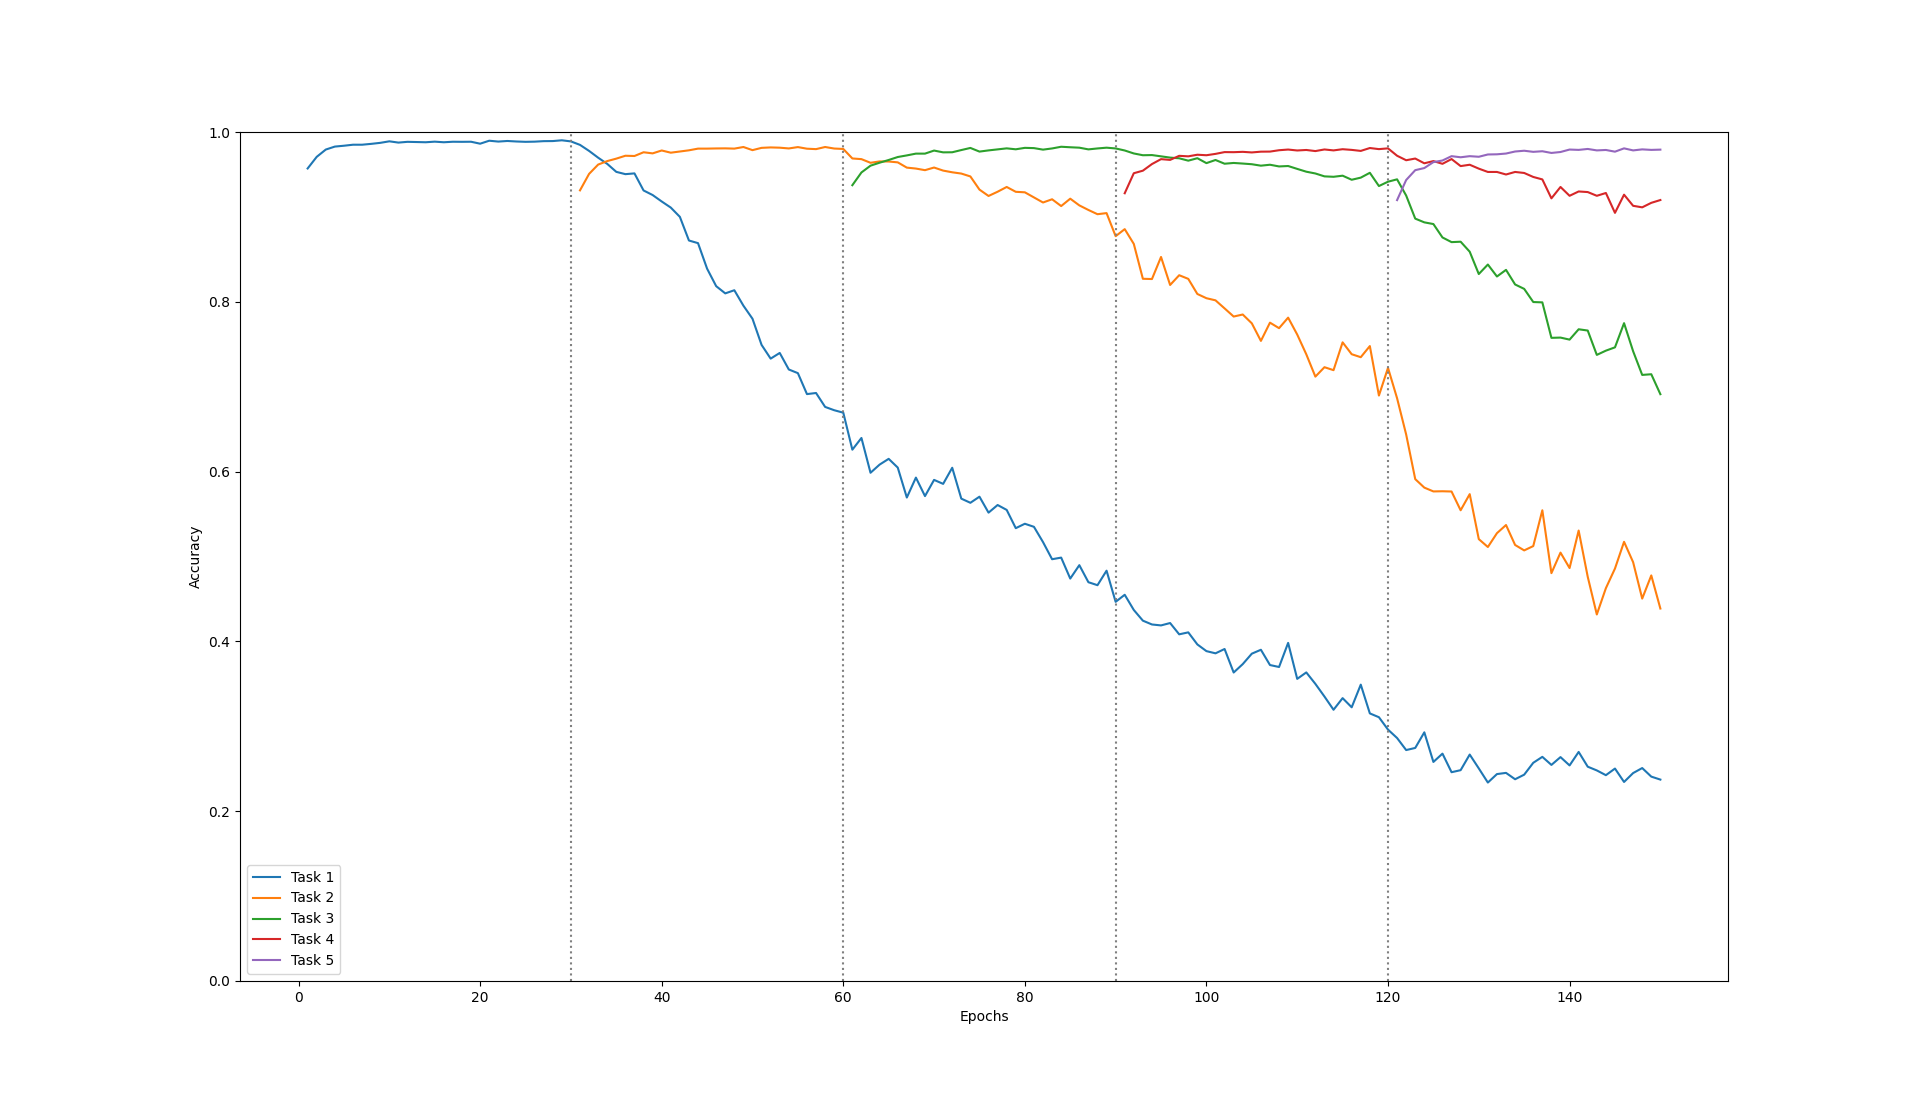
\includegraphics[width=\textwidth]{figures/exp0_results.png}
                \caption{\textit{Clearly, this is why it is called
                \textbf{catastrophic} forgetting. As soon as the network 
                is trained on a new task, performance drops significantly. 
                While a lot better than chance, the accuracy on the first 
                task drops from almost 100\% to a mere 60\% after training 
                on the second one. On the MNIST dataset, the accuracy for 
                random guessing would be 10\%.}}
            \end{figure}
        \subsection*{Incremental training with penalty for each task}
            \begin{figure}[H]
                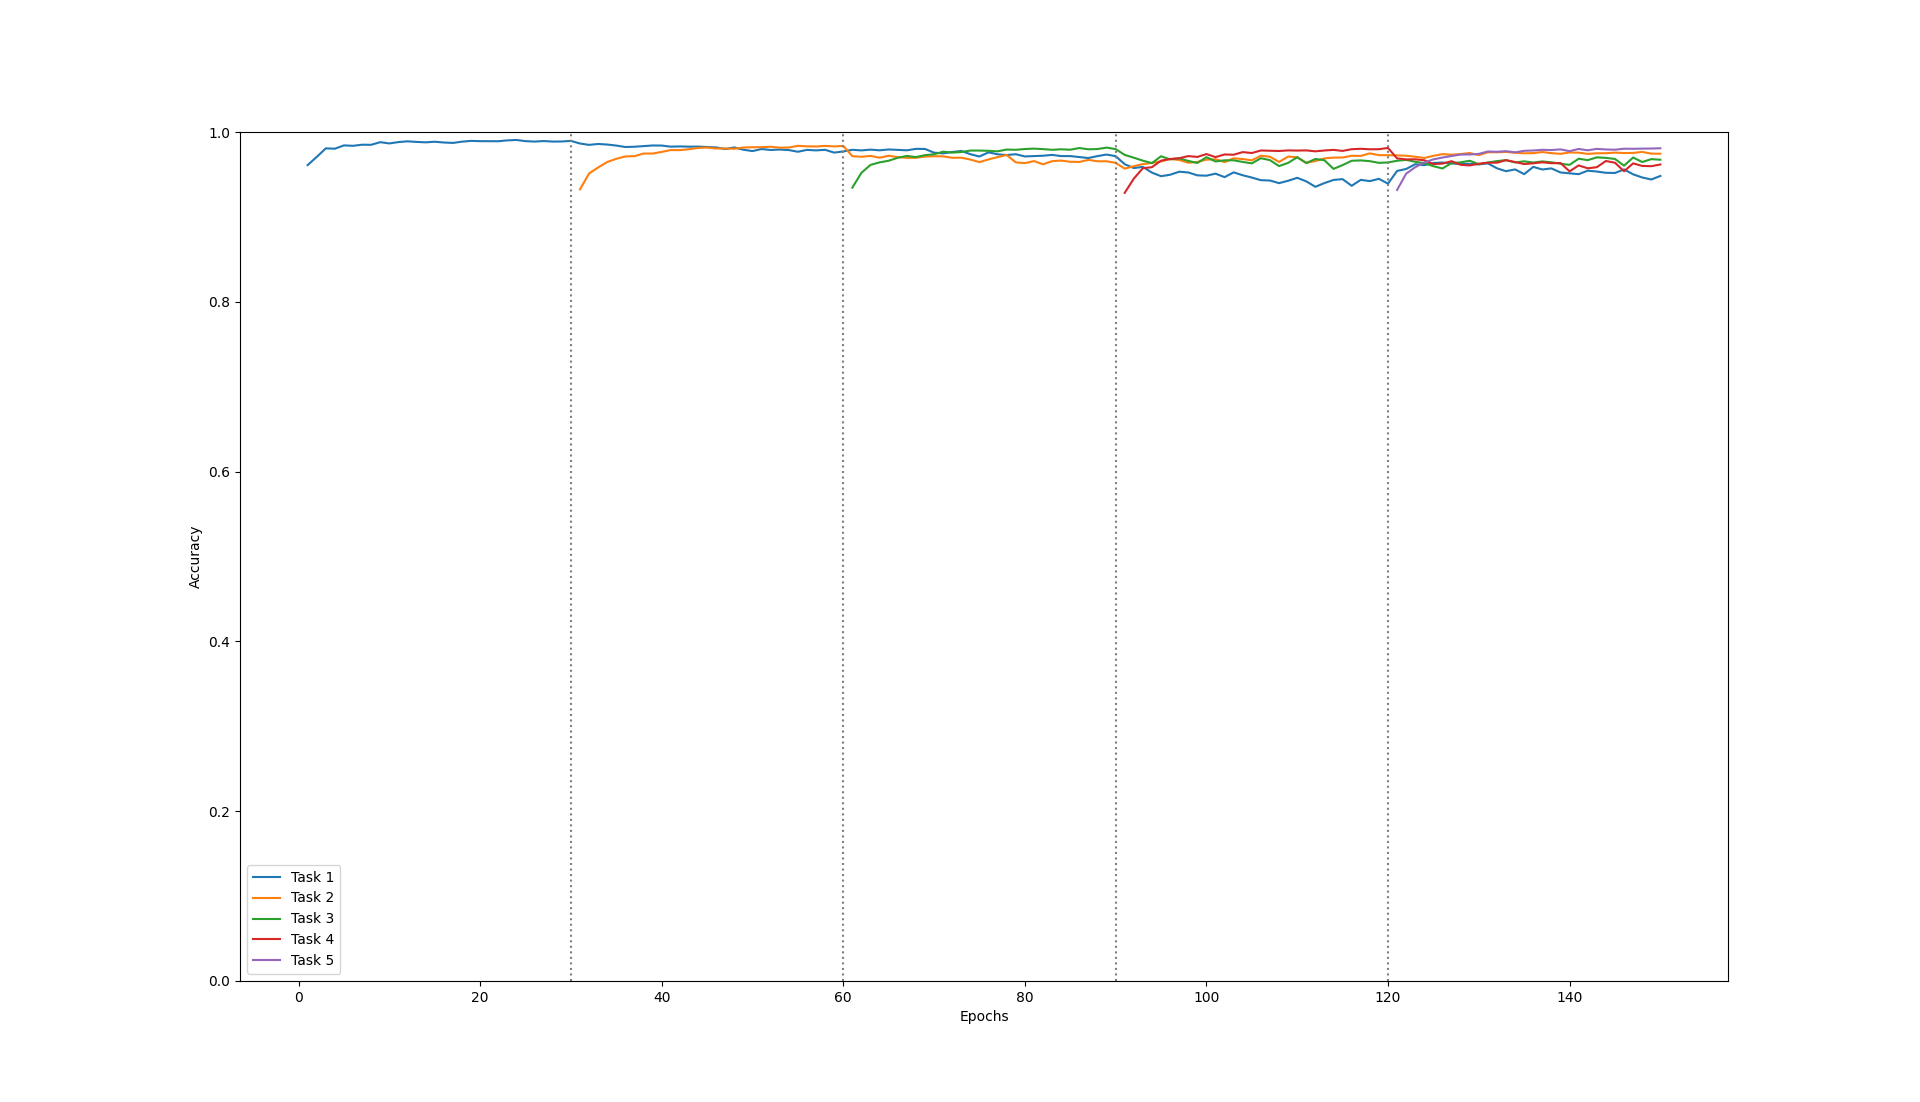
\includegraphics[width=\textwidth]{figures/exp1_results.png}
                \caption{\textit{Performance is high on all tasks. While the 
                network always performs best on the most recently trained task,
                this does not seem to hold over longer time periods. For example, 
                at the end, the network performs better on task 2 (orange) than 
                on task 4 (red) which it was trained on more recently.}}
            \end{figure}
        \subsection*{Incremental training with penalty for previous task}
            \begin{figure}[H]
                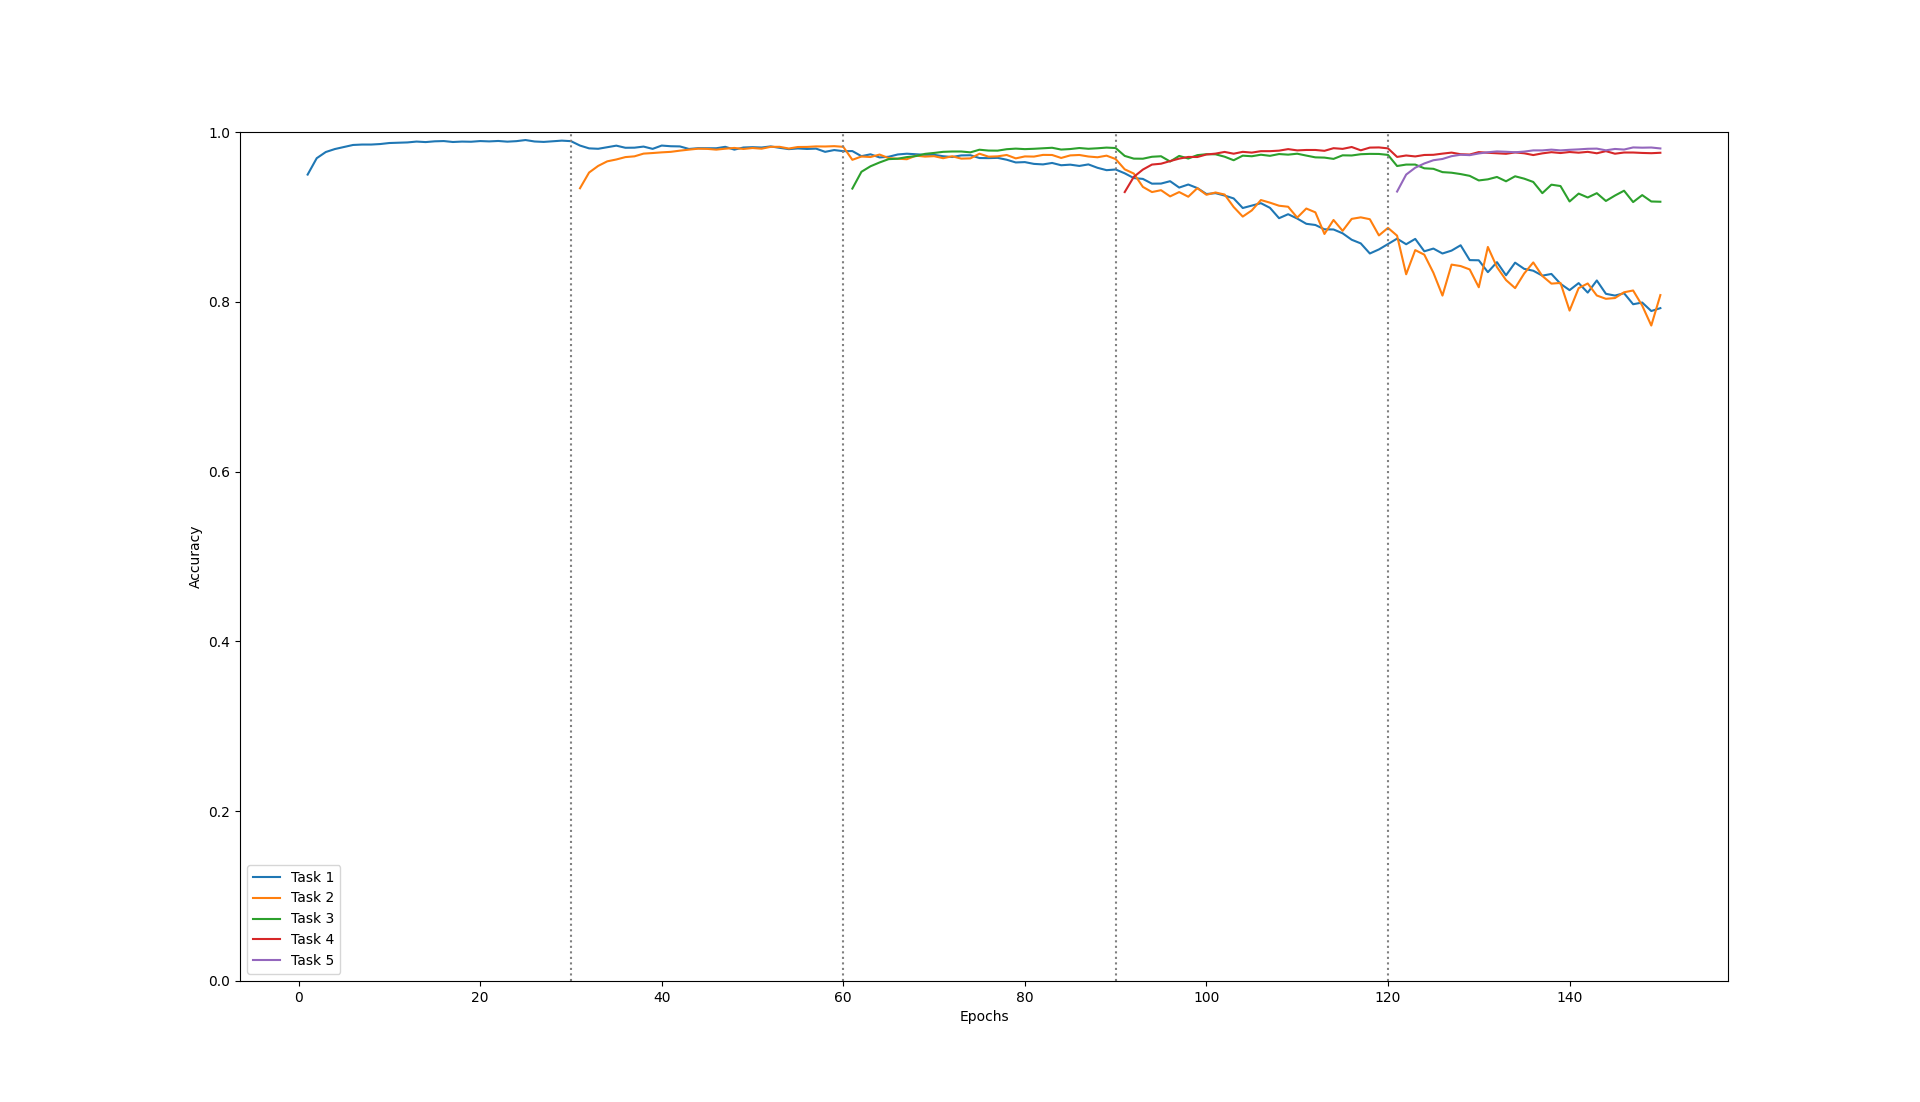
\includegraphics[width=\textwidth]{figures/exp2_results.png}
                \caption{\textit{Performance on a task degrades significantly 
                after adding two or three additional tasks. There is also 
                a lot of fluctuation in accuracy on the older tasks.}}
            \end{figure}
    \section*{Discussion}
        \subsection*{Performance analysis}
            Using an EWC penalty associated with all previously learned 
            tasks, rather than only the most recently learned one, clearly offers 
            the best and most consistent performance. Interestingly though, for 
            a limited number of tasks, a penalty for only the most recent task 
            still offers relatively high accuracy. It is far better from an 
            accuracy point of view than the network trained without any EWC at all.

            Presumably, the reason for this is that the EWC penalty associated 
            with remembering task $i$ still embeds a preference for parameter 
            values similar to those learned for task $i-1$, even if there is no 
            explicit reference to those values when computing the penalty. 
            It is perhaps a little surprising that the effect is so strong, 
            since EWC only encourages staying close to previously trained weights
            if they are important to that task. After all, there is no guarantee that 
            the weights that are important for task $i$ were also important for 
            task $i-1$. One might even expect the opposite to be the case: 
            because the network is encouraged to not change the weights 
            important for task $i-1$, the most efficient way to train it for 
            task $i$ might be to more or less leave those particular weights alone 
            unchanged and rely on other ones.

        \subsection*{Convolutional neural network \& pixel-permutations}
            One may question whether the pixel-permuted dataset is reasonable
            for evaluating a convolutional neural network. The purpose of the 
            convolutional layers is to recognize and exploit spacial localities 
            in the images. These local features are certainly impacted by shuffling 
            all pixels randomly across the image. This topic is explored further,
            for example in \cite{ivan2019convolutional}.
            
            It might have been more reasonable to permute the MNIST dataset in a way 
            that somewhat preserves spacially local features of the image. One 
            suggestion is to divide the images into (square) sub-images, e.g. 
            dividing the 28x28 image into 16 7x7 squares and permuting the 
            position of those squares within the image:

            \begin{figure}[H]
                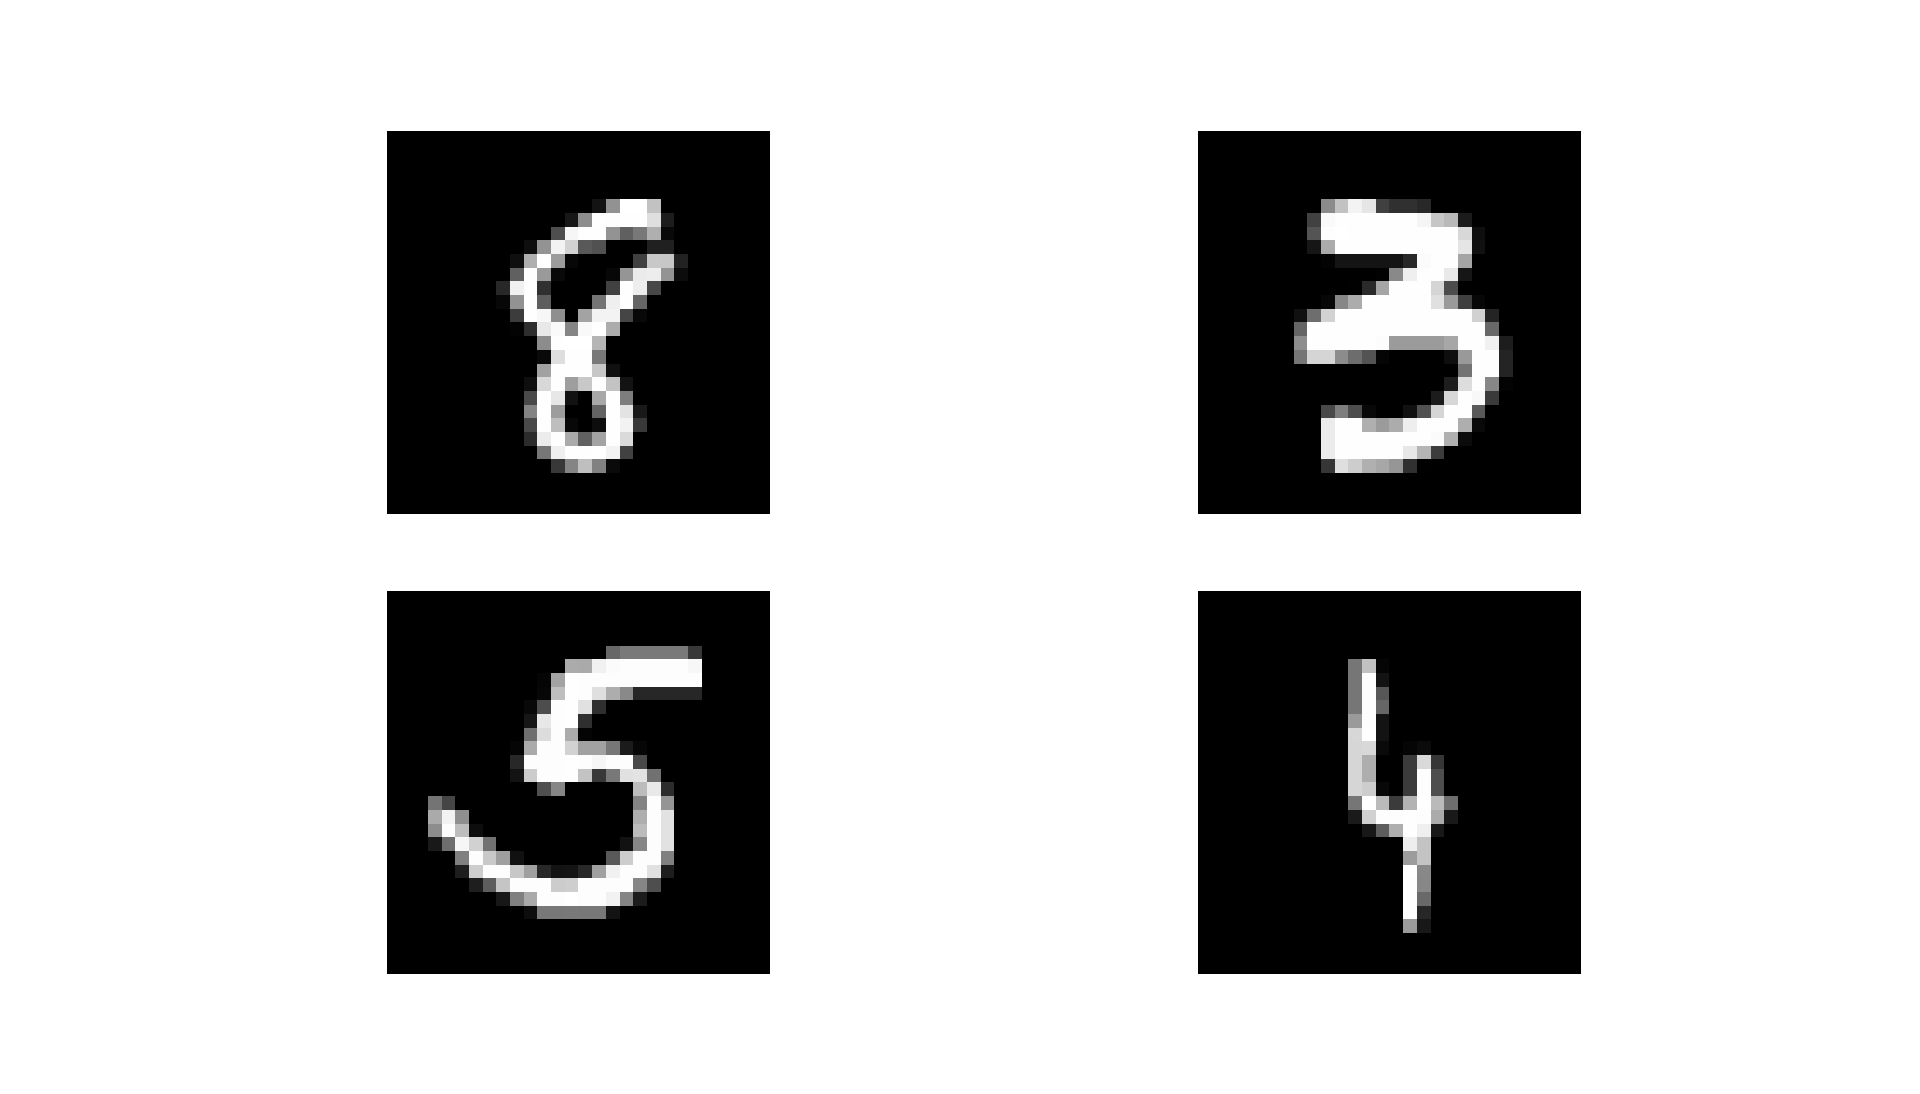
\includegraphics[width=0.49\textwidth]{figures/regular_mnist.png}
                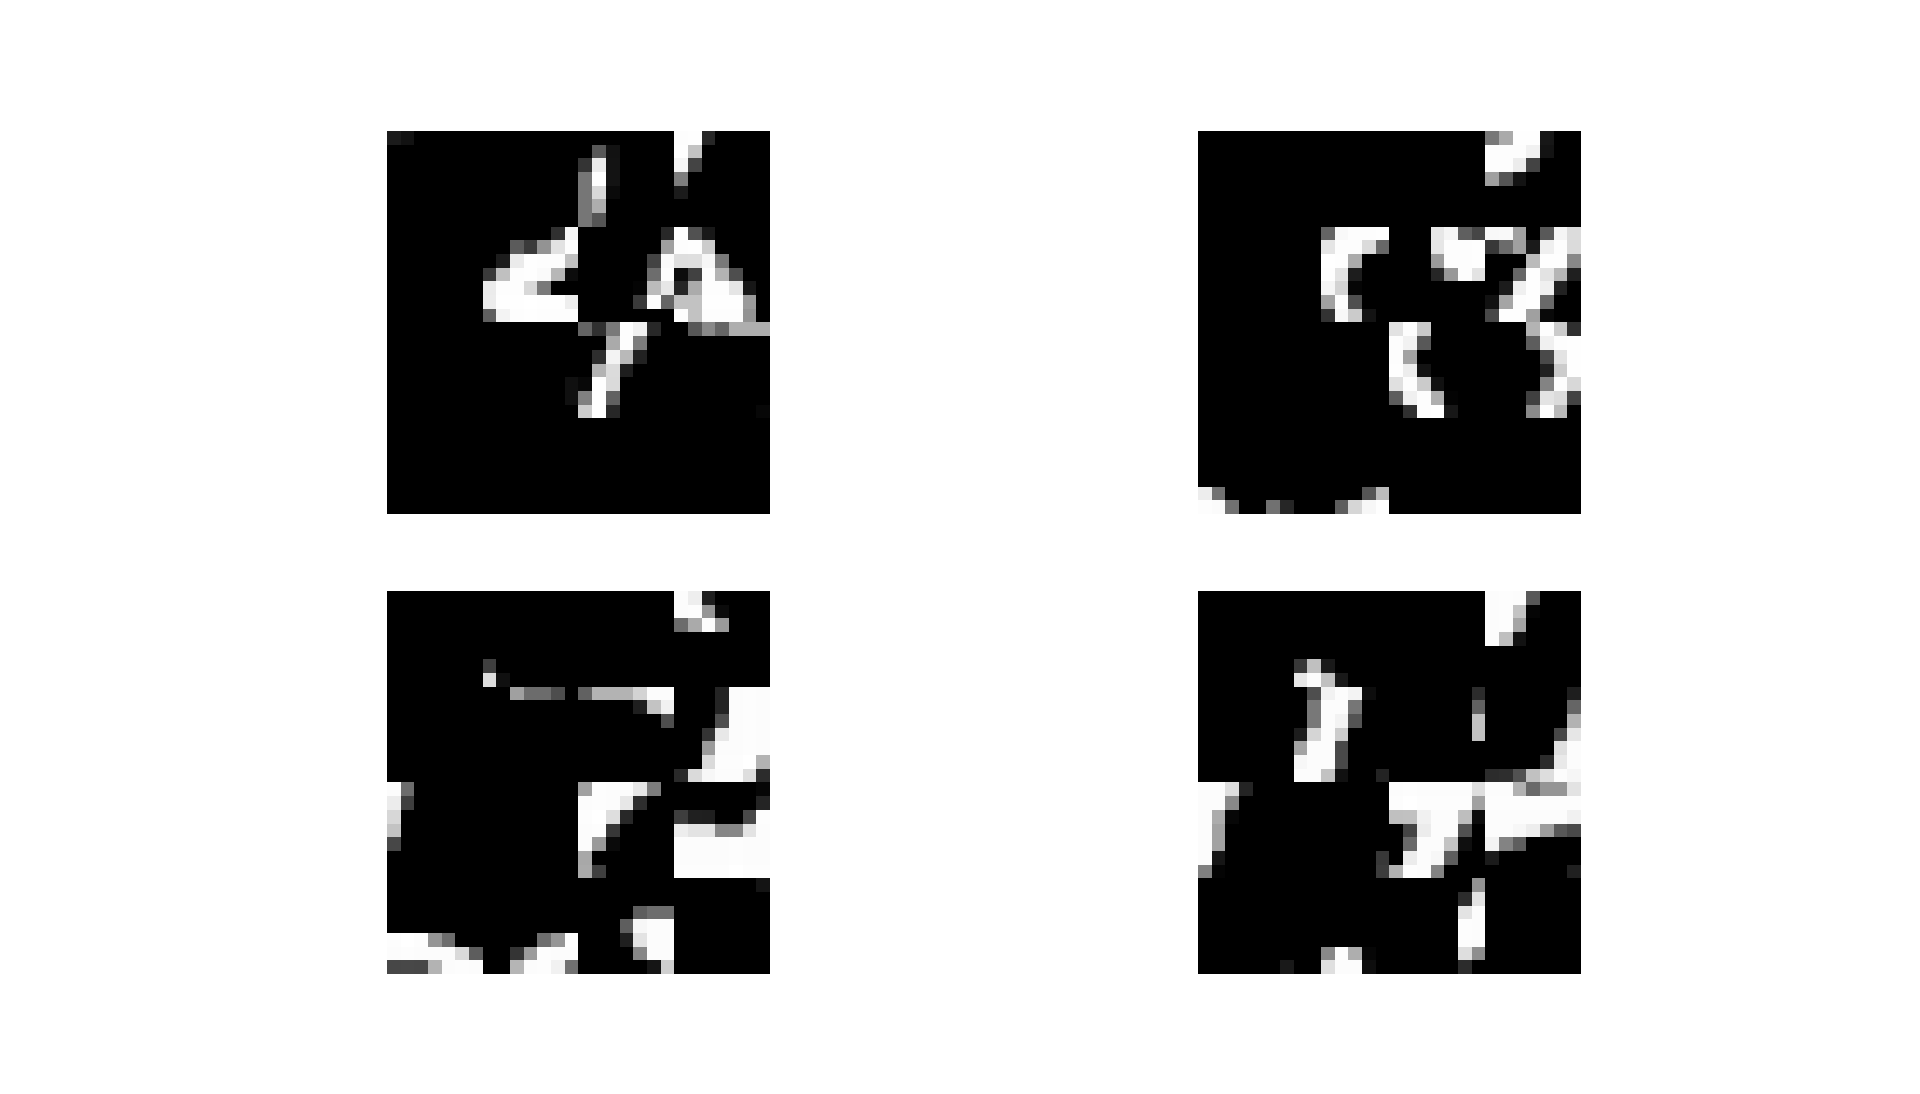
\includegraphics[width=0.49\textwidth]{figures/shuffled_mnist.png}
                \caption{\textit{To the left, random images from the MNIST dataset. 
                To the right, random images from an MNIST dataset where the 
                7x7 sub-squares have swapped positions. Clearly this kind of 
                permutation preserve some spacially local features such as lines,
                but may divide them into several pieces and/or change their 
                position within the image. N.b. the permuted images to the right 
                are not permutations specifically of the images to the left.}}
            \end{figure}

            One may even argue that in these experiments, the convolutional 
            layer limits performance on the permuted datasets, because the 
            structures it learns to recognize on the original MNIST dataset 
            (presumably lines and other simple geometric shapes) 
            cannot be used meaningfully on the permuted ones. 
            Perhaps, a fully connected neural network could be used for these 
            tasks instead. Obviously, for image recognition tasks that are more 
            complicated, CNN:s offer far better performance. It could be interesting  
            to experiment a pre-trained model like VGG16, freezing some or all of 
            the convolutional layers and apply EWC on the other ones, and see how 
            well it can adapt to different image recognition tasks.

        \subsection*{Impact on training time}
            Training a network with EWC is not noticeably slower than using any 
            other regularization function. Between tasks, the fisher diagonal 
            has to be computed and the trained paramters saved. This entails a 
            small performance hit. The time spent saving traind parameters 
            and computing Fisher diagonals is proportional to the size of the 
            network and the number of tasks trained on. While the computation 
            of the Fisher diagonal is by no means quick, it is 
            (for reasonably large networks) overshadowed by the time spent in
            actual training.
            
            Obviously, the time spent computing the regularization penalty is 
            proportional to the number of tasks that have been trained already, 
            as there is one term associated with each task. It is possible to 
            avoid this, however. Noting that:

            \begin{equation*}
                \begin{split}
                & \sum_{K}{\sum_{i}{F_{K,i}(\theta_i - \theta_{K,i})^2}} \\ &= \\
                &    \sum_{i}{
                        \left[\theta_i^2\left({\sum_{K}{F_{K,i}}}\right) -  
                        \theta_i \left(\sum_{K}{F_{K,i}\theta_{K,i}}\right)\right]} + 
                        \sum_{i}{\sum_{K}{F_{K,i}\theta_{K,i}^2}} 
                \end{split}
            \end{equation*}

            it would be possible to, at the end of training for each task, 
            compute the quantities 

            \begin{equation*}
                \Sigma_{1,i} = \sum_{K}{F_{K,i}}\quad, \quad
                \Sigma_{2,i} = \sum_{K}{F_{K,i}\theta_{K,i}}\quad \text{and} \quad
                \Sigma_3 = \sum_{i}\sum_{K}{F_{K,i}\theta_{K,i}^2}
            \end{equation*}
            
            for each $i$. Note that this simply amounts to adding the values 
            \begin{equation*}
                \sigma_{1,i} = F_{K^*,i}\quad, \quad
                \sigma_{2,i} = F_{K^*,i}\theta_{K^*,i}\quad \text{and} \quad
                \sigma_3 = \sum_{i}{F_{K^*,i}\theta_{K^*,i}^2}
            \end{equation*}
            computed from the most recently learned task $K^*$ onto the 
            quantities $\Sigma_{1,i}$, $\Sigma_{2,i}$ and $\Sigma_3$ 
            (that are continously updated after learning each task).

            The penalty could then be computed as 

            \begin{equation*}
                \frac{\lambda}{2}
                \left(\sum_{i}{\left[\theta_i^2\cdot\Sigma_{1,i} - 
                \theta_i\cdot\Sigma_{2,i}\right]} + 
                \Sigma_3\right)
            \end{equation*}

            Which is linear in the amount of parameters instead of linear
            in the amount of parameters multiplied by the number of tasks 
            learned.



    \clearpage
    \bibliography{sources}
    \clearpage
    \begin{appendices}
    \section{Network architecture \& parameters}
    \label{appendix:architecture}
    For all experiments, the following Keras sequential model was used:
    \begin{lstlisting}
    model = tf.keras.models.Sequential([
        tf.keras.layers.Input(shape=(28,28,1), name='input'),
        tf.keras.layers.Dropout(rate=0.2, name='dropout1'),
        tf.keras.layers.Conv2D(
            64, 
            (3, 3),
            padding='same',
            activation='relu',
            name='conv1-1'
        ),
        tf.keras.layers.MaxPooling2D(
            pool_size=(2,2),
            name='pool1'
        ),
        tf.keras.layers.Flatten(),
        tf.keras.layers.Dense(
            1024, 
            activation='relu',
            name='fc1'
        ),
        tf.keras.layers.Dropout(rate=0.5, name='dropout2'),
        tf.keras.layers.Dense(
            1024, 
            activation='relu', 
            name='fc2'
        ),
        tf.keras.layers.Dropout(rate=0.5, name='dropout3'),
        tf.keras.layers.Dense(
            10, 
            activation='softmax',
            name='output'
        )
    ])
    \end{lstlisting}

    Training parameters were:
    \begin{center}
        \begin{tabular}{ |l||c| } 
            \hline
            Training epochs (per task) & 30 \\ 
            \hline
            Batch size & 64 \\
            \hline
            Learning rate & $10^{-4}$ \\ 
            \hline
            $\lambda$ used for EWC & 200 \\
            \hline
            Keras optimizer & ADAM \\
            \hline
            Keras loss function & Categorical Crossentropy \\
            \hline
        \end{tabular}
    \end{center}

    \end{appendices}
\end{document}